%%%%%%%%%%%%%%%%%%%%%%%%%%%%%%%%%%%%%%%%%%%%%%%%%%%
%% P3: Phenomenology of Particle Physics                         
%%
%% Author:  André Rubbia                   		 
%%
%% Figure 28.1 Schematic layout of a wide-band and narrow-band neutrino beam.
%%
%% This work is licensed under the Creative Commons Attribution 4.0 International License. 
%% To view a copy of this license, visit http://creativecommons.org/licenses/by/4.0/ or 
%% send a letter to Creative Commons, PO Box 1866, Mountain View, CA 94042, USA.
%%
%%%%%%%%%%%%%%%%%%%%%%%%%%%%%%%%%%%%%%%%%%%%%%%%%%%

\documentclass[a4paper,10pt]{article}

\usepackage[T1]{fontenc}
\usepackage[utf8]{inputenc}
\usepackage{lmodern}
\usepackage[labelfont=bf]{caption}
\usepackage{upgreek}

\usepackage{tikz}
\usepackage{pgfplots}
\pgfplotsset{compat=1.17}
\usepgfplotslibrary{ternary}
\usepgfplotslibrary{fillbetween}
\usepgfplotslibrary{external}

\def\d{\mathrm{d}}
\setlength{\oddsidemargin}{-1.0cm}
\setlength{\evensidemargin}{-1.0cm}
\setlength{\textheight}{25cm}
\setlength{\textwidth}{18cm}

\pgfkeys{/pgf/number format/.cd,1000 sep={}}

\begin{document}

%%%%%%%%%%%%%%%%   FIGURE  %%%%%%%%%%%%%%%%%%%%%%%%%%%%%%
\begin{figure}[htbp]
\centering
\begin{tikzpicture}[scale=0.9]
	\begin{scope}[shift={(0,0)}]

% shield + decay tunnel
\draw[gray,thick,fill opacity=0.2,fill=gray] (0,-2) rectangle +(7,4);
\draw[gray,thick] (0,-0.5) rectangle +(3,1);
\draw[white,thick,fill=white] (-0.1,-0.45) rectangle +(3.05,0.9);

% neutrino detector
\draw[gray,thick,fill opacity=0.2,fill=gray] (8,-2.5) rectangle +(1,5);

% symmetry axis
\draw[blue,thick,dashed] (-1,0) -- +(11,0);
% decay path of neutrino
\draw[blue,thick,dashed] (1.5,0) -- +(7,2);

% flux monitors
\draw[black,thick,fill=black] (3.2,-0.4) rectangle +(0.02,0.8);
\draw[black,thick,fill=black] (3.4,-0.4) rectangle +(0.02,0.8);
\draw[black,thick,fill=black] (3.6,-0.4) rectangle +(0.02,0.8);

% decay and interaction points
 \draw[very thick, fill=black] (1.5,0) circle (0.05);
 \draw[very thick, fill=black] (8.5,2) circle (0.05);
 \node[above] at (1.5,0) {$D$};
 \node[above] at (8.5,2) {$I$};

 % distances
 \draw[magenta,very thick, <->] (1.5,3) -- (8.5,3);
 \draw[magenta,very thick, <->] (8.5,0) -- (8.5,2);
 \node[magenta,above] at (5,3) {$L$};
 \node[magenta,right] at (8.5,1) {$R$};
\draw[very thick,->,red] (6,0.) arc (0:12:6);
 \node[red,left] at (6,0.5) {$\theta_\nu\approx R/L$};

 \node[right] at (0,-0.3) {\small Decay tunnel};
\node[right] at (4.75,-1.75) {\small Muon shield};
\node at (8.5,-2.75) {Neutrino detector};
\node at (3.35,-0.675) {\small Flux monitors};
	\end{scope}

	\draw[blue,thick,dashed] (-2,2) -- (-1,0);
	\draw[blue,thick,dashed] (-2,-2) -- (-1,0);

%% WIDE BAND BEAM
	\begin{scope}[shift={(-4.5,2)}]
		\draw[blue,thick,dashed] (0,0) -- +(2.5,0);
		\draw[black,thick,fill=black] (-0.5,-0.15) rectangle +(0.3,0.3);
		\draw[red,thick, ->] (-1.6,0,0) -- +(1,0);
		\node at (-1,-0.5) {\tiny High energy};
		\node at (-1,-0.75) {\tiny proton};
		\node at (-1,-1) {\tiny  beam};
		\node at (-0.275,0.4) {\tiny  target};
		\begin{scope}[shift={(0.5,0)}]
			\draw[fill=white] (0,-0.5) .. controls (-0.2, 0) .. (0,0.5) -- (0,0.5) .. controls (0.2, 0) .. (0,-0.5);
		\end{scope}
		\begin{scope}[shift={(1.75,0)},scale=1.2]
			\draw[fill=white] (0,-0.5) .. controls (-0.2, 0) .. (0,0.5) -- (0,0.5) .. controls (0.2, 0) .. (0,-0.5);
		\end{scope}
		\node at (1.15,-0.75) {\tiny Focusing};
		\node at (1.15,-1) {\tiny sign selection};
		\node at (1.15,-1.25) {\tiny of $\pi$,$K$};
		\node at (0.3,1.2) {Wide-band neutrino beam};
	\end{scope}

%% NARROW BAND BEAM
	\begin{scope}[shift={(-4.5,-1.5)}]
		\draw[blue,thick,dashed] (0,0) -- +(1.25,0);
		\draw[blue,thick,dashed] (1.25,0) -- +(1,-0.5);
		\draw[gray,thick,dotted] (2.25,-0.5) -- +(0.25,0);
		\draw[black,thick,fill=black] (-0.5,-0.15) rectangle +(0.3,0.3);
% momentum slit
		\draw[black,thick,fill=black] (1.7,-0.05) rectangle +(0.02,0.5);
		\draw[black,thick,fill=black] (1.7,-0.9) rectangle +(0.02,0.5);
%
		\draw[red,thick, ->] (-1.6,0,0) -- +(1,0);
		\node at (-1,-0.5) {\tiny High energy};
		\node at (-1,-0.75) {\tiny proton};
		\node at (-1,-1) {\tiny  beam};
		\node at (-0.275,0.4) {\tiny  target};
		\begin{scope}[shift={(0.5,0)}]
			\draw[fill=white] (0,-0.5) .. controls (-0.2, 0) .. (0,0.5) -- (0,0.5) .. controls (0.2, 0) .. (0,-0.5);
		\end{scope}
		\begin{scope}[shift={(1,0)}]
			\draw[fill=white] (0,-0.5) -- (0.25,0.5) -- (0.5,-0.5) -- (0, -0.5);
		\end{scope}
		\begin{scope}[shift={(2.45,-0.5)}, rotate=180]
			\draw[fill=white] (0,-0.5) -- (0.25,0.5) -- (0.5,-0.5) -- (0, -0.5);
		\end{scope}
		\begin{scope}[shift={(0,-0.5)}]
		\node at (1.15,-0.75) {\tiny Momentum and};
		\node at (1.15,-1) {\tiny sign selection};
		\node at (1.15,-1.25) {\tiny of $\pi$,$K$};
		\node at (0.3,1.5) {Narrow-band neutrino beam};
		\end{scope}
	\end{scope}
\end{tikzpicture}
\caption{Schematic layout of a wide-band and narrow-band neutrino beam.
$D$ represents the meson decay point and $I$ the neutrino
	interaction point. It is assumed that $L\gg R$.}
\end{figure}
%
%%%%%%%%%%%%%%%%   END FIGURE  %%%%%%%%%%%%%%%%%%%%%%%%%%%%%%
%


\end{document}
